%!TEX root = ../thesis.tex
\chapter{紡織染色製程現況}
\label{c:description}
一般而言染色製程總成本分為生產成本及品質成本。生產成本包括染整過程中之水、電成本及實驗室先期的實驗成本,染整過程中,若想要提高良率,通常現場所需要的生產成本也隨之提高。另一項成本為品質成本,當良率下降時導致色差、顏色不均、波紋及固色率不到標準,未達對色率標準時,不良品需再經過漂洗、補色等流程或直接報廢,這些過程產生的成本稱為品質成本。當良率愈低也就是重複染整的次數相對變多,對此造成資源上及時間的浪費,因此品質成本大幅增加。但是相對的,如果良率提升,會使得品質成本下降,但卻會造成生產成本大幅增加。生產成本與品質成本可能的相對應關係如圖~\ref{fig:graph1}所示,但如果能夠找出能夠品質與成本兼具的染整製成組合,如圖~\ref{fig:graph1}中的最佳製程總成本的位置,則必須要跳脫過去常用的製程參數,才有可能達到,但在求得製程參數組合的過程中,只依靠回饋去搜尋,則需要大量的實驗成本才有可能達到。
\begin{figure} 
\centering  
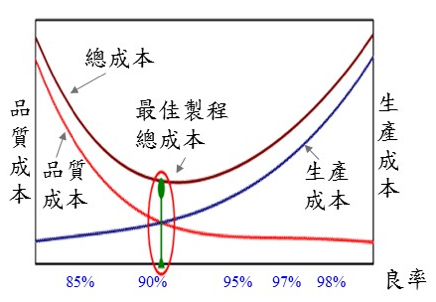
\includegraphics[width=8cm,height=6cm]{Graph/graph1.png}
\caption{染整製程品質成本及生產成本之關係曲線現況描述}
\label{fig:graph1}
\end{figure}